%!TEX root = ../thesis.tex

\chapter{Projekt \projectname{}}

In diesem Kapitel soll die Grundlage der praktischen Arbeit, welche im folgenden \projectname{} genannt wird, erläutert werden.

\section{Motivation}
\label{sec:motivation}

Monitoring Tools dienen der Übewachung und Kontrolle bestehender Softwareprodukte.
Ein Software-System beinhaltet diverse Abläufe und Metriken, welche geprüft und ausgewertet werden können, um Entwicklern und Systemadministratoren
aussagekräftige Einsicht in ihre Systeme zu gewähren. Speziell nach der Veröffentlichung eines Projektes oder neuer Patches
ist es meist unabdingbar, das aktualisierte System hinsichtlich Stabilität und Performance kritisch zu beobachten. Ein weiterer Aspekt, den es zu überwachen gilt,
ist die Skalierfähigkeit eines Produktes. Steigt die Aktivität einer Applikation, beispielsweise durch steigende Nutzerzahlen,
muss sichergestellt werden, dass steigende Antwort- und Ausfallzeiten schnell erkannt und richtig interpretiert werden, damit Skalierungsprobleme schnellstmöglich behoben werden können.

Handelt es sich bei dem zu überwachenden System um ein komplexes Zusammenspiel diverser Microservices, gestaltet sich die Herausforderung der manuellen Überwachung, beispielsweise anhand
Serverlogs, deutlich schwieriger.

Innerhalb einer Microservice Architektur ist es nicht notwendig, dass alle Services auf einem gemeinsamen Server operieren.
Es ist möglich dass Services auf einer Vielzahl von Servern möglicherweise an komplett unterschiedlichen geographischen Punkten miteinander agieren,
oder im Problemfall nicht miteinander agieren können. Instanzen einzelner Services können zur Laufzeit starten, stoppen oder abstürzen
und sollten dennoch den reibungslosen Ablauf der Applikation nicht behindern. Microservice Architekturen sind also deutlich komplexer zu überblicken, da durch die Verteilung von Funktionalität auch
mögliche Fehlerquellen verteilt werden.
Daher ist ein Monitoring Tool, um Stabilität und Performance einer solchen Architektur zu gewährleisten, meist stark sehr sinnvoll.

\newpage

\section{Anforderungsanalyse}
\label{sec:anforderungsanalyse}
Im Folgenden werden Anforderungen an den Prototypen, welcher im Rahmen der Bachelorarbeit entwickelt wird, gestellt.
Der Prototyp soll den in \ref{sec:motivation} Motivation beschriebenen Sachverhalt vereinfachen.
Innerhalb dieser Arbeit wird das Frontend-System konzipiert und implementiert.
Instrumentationen der zu prüfenden Systeme sowie die Implementierung des Backend-Systems wird in der Bachelorarbeit \emph{
Design and implementation of a SaaS-monitoring application for distributed systems} von Timo Weiß behandelt.

\subsection{Views}

Dieses Kapitel ist in Unterkapitel unterteilt, welche den einzelnen Views der Applikation \projectname{} entsprechen.
In diesen werden Anforderungen beschrieben sowie mithilfe von Mock Screenshots visuell aufbereitet.

\subsubsection{Login / Registrieren}

Dieser Screen erscheint, wenn die Applikation erfolgreich geladen wurde und der Nutzer nicht eingeloggt ist.
Nutzer können sich mit bestehenden Accounts einloggen (Abbildung \ref{fig:login}) oder neu registrieren (Abbildung \ref{fig:register}).
Rudimentäres Error-Handling weist Nutzer auf fehlerhafte Eingaben hin.

Nach erfolgreichem Login beziehungsweise nach erfolgreichem Registrierungsvorgang werden Nutzer auf die Ansicht \emph{System wählen / erstellen} weitergeleitet.

\vspace{0.3cm}

\begin{figure}[h]
 \centering
 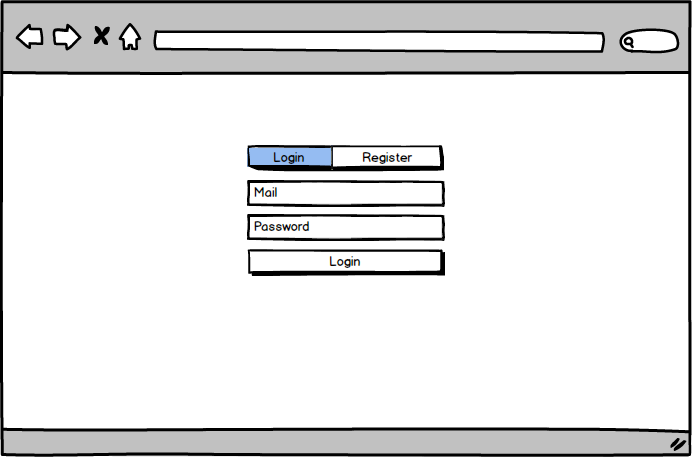
\includegraphics[width=0.7\linewidth]{kapitel1/mocks/Login.png}
 \caption{Login Screen Mock}
  \label{fig:login}
\end{figure}

\begin{figure}[h]
 \centering
 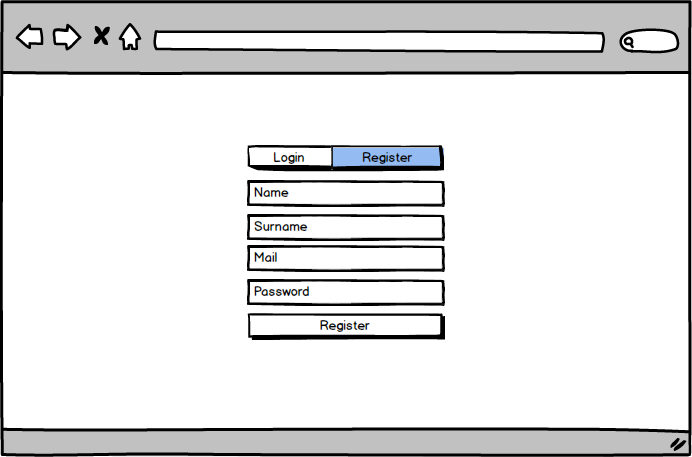
\includegraphics[width=0.7\linewidth]{kapitel1/mocks/Register.png}
 \caption{Register Screen Mock}
  \label{fig:register}
\end{figure}


\textbf{Eingabefelder Login Formular}
\begin{itemize}
\item Mail (String, valide Mailadresse, eindeutig im System)
\item Password (String)
\end{itemize}

\textbf{Eingabefelder Register Formular}
\begin{itemize}
\item Name (String)
\item Surname (String)
\item Mail (String, valide Mailadresse, eindeutig im System)
\item Password (String)
\end{itemize}



\subsubsection{System wählen / erstellen}

Nutzer können mithilfe von \projectname{} mehrere verschiedene Anwendungen monitoren.
Daher wird eine Übersichtsseite (Abbildung \ref{fig:system-picker}) benötigt
um ein aktives System zu definieren. Zusätzlich soll auf dieser Ansicht die Möglichkeit bestehen neue Systeme anzulegen.

\vspace{0.3cm}

\begin{figure}[h]
 \centering
 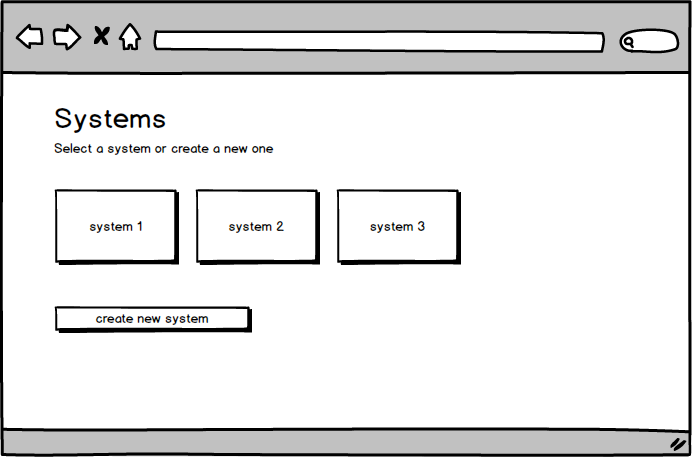
\includegraphics[width=0.6\linewidth]{kapitel1/mocks/system-picker.png}
 \caption{System wählen Mock}
 \label{fig:system-picker}
\end{figure}


\subsubsection{Dashboard}

Auf dem Dashboard soll der Nutzer die wichtigsten Informationen über sein System erhalten.
Fehlerverhalten des Systems und fehlerhafte Konfigurationen sollen deutlich und informativ dargestellt werden.
Zusätzlich soll das Dashboard als Einstiegspunkt für weitere Ansichten der Anwendung dienen.

\subsubsection{Metriken}

Die Metriken-Sektion soll eine Kollektion von Diagrammen beinhalten.
Dabei soll die Applikation und der aktive Beobachtungszeitraum gewählt werden können.

\begin{figure}[h]
 \centering
 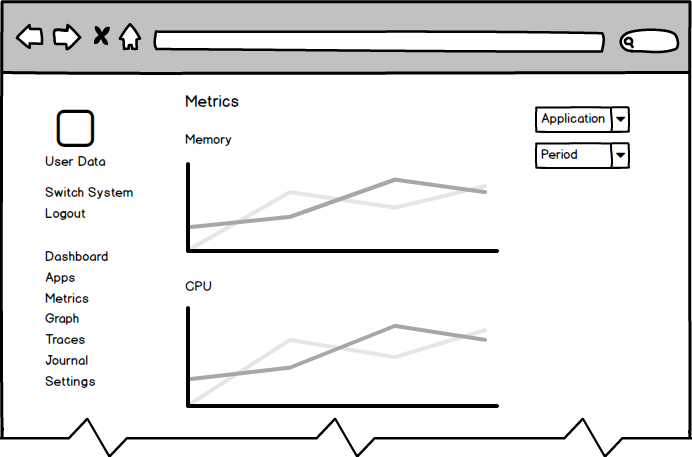
\includegraphics[width=0.6\linewidth]{kapitel1/mocks/metrics.png}
 \caption{Metrik Mock}
  \label{fig:metrics}
\end{figure}

\textbf{Diagramme}

\begin{itemize}
\item CPU Load
\item Memory
\item Requests client send
\item Requests server receive
\end{itemize}


\subsubsection{Graph}

Im Vergleich zur Metriken-View soll der Graph nicht nur einzelne Applikationen darstellen,
sondern das Kommunikationsnetz des Gesamtsystems visualisieren.
Wie in Abbildung \ref{fig:graph} veranschaulicht, sollen dabei Services als Knoten und Requests als Kanten dargestellt werden.
Bei den zu visualisierenden Metriken handelt es sich um die Faktoren Anzahl und Dauer der Requests zwischen den Services.
Zusätzlich soll erneut die Möglichkeit bestehen, den Beobachtungszeitraum zu definieren.

\begin{figure}[h]
 \centering
 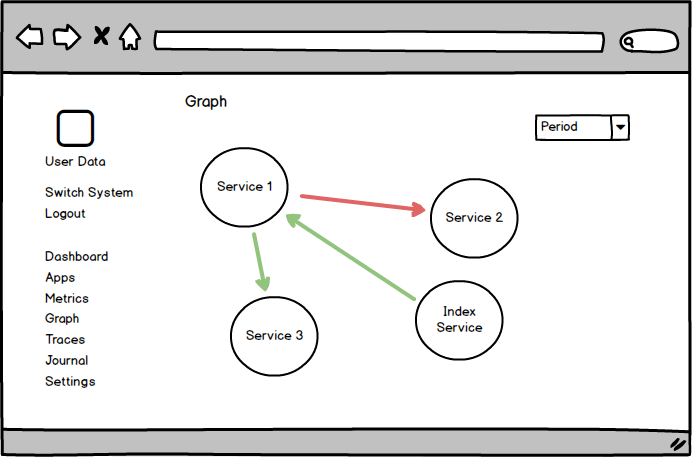
\includegraphics[width=0.6\linewidth]{kapitel1/mocks/graph.png}
 \caption{Graph Mock}
 \label{fig:graph}
\end{figure}

\subsubsection{Traces}

Die Traces Sektion besteht aus zwei verschiedenen Ansichten. Die Übersichtsliste der Request Einstiegspunkte,
leitet zur Trace Detailseite (Abbildung \ref{fig:trace}) über. Im Detail besteht ein Trace aus den Requests
aller an einer Aktion beteiligten Services. Dabei werden die Service-Zugriffe in Relation zur Zeit in einem Gantt Chart dargestellt.

\vspace{0.3cm}
\begin{figure}[h]
 \centering
 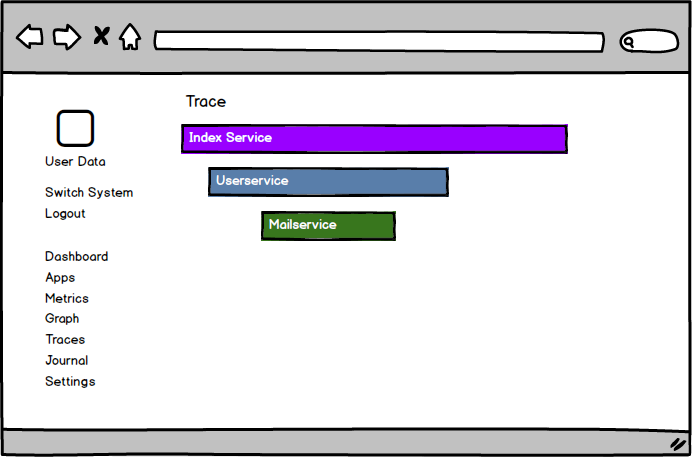
\includegraphics[width=0.7\linewidth]{kapitel1/mocks/trace.png}
 \caption{Trace Detailseite Mock}
 \label{fig:trace}
\end{figure}


\subsubsection{Journal}

\begin{figure}[h]
 \centering
 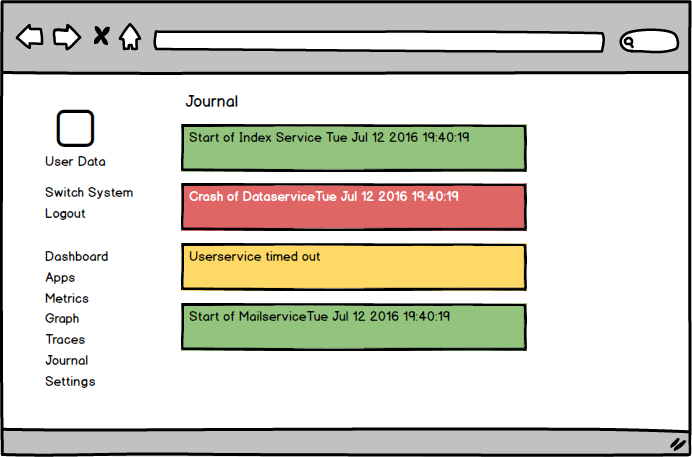
\includegraphics[width=0.7\linewidth]{kapitel1/mocks/journal.png}
 \caption{Journal Mock}
 \label{fig:journalmock}
\end{figure}

Das Journal (Abbildung \ref{fig:journalmock}) beinhaltet Einträge bezüglich Serverstart, Serverstop und Servercrash.


\newpage

\subsection{Plattformen}

Applikationen können anhand von Diagrammen und Graphen im Detail analysiert werden,
ferner möchte ein Nutzer reaktiv über Vorgänge seines Systems informiert werden, speziell wenn Latenzprobleme und Service-Ausfälle reibungslose Abläufe eines Systems gefährden.
Hierzu erhält der Nutzer Notifications über das Event System.

Die Applikation soll daher als App für iOS und Android sowie als Desktop Applikation für MacOS, Linux und Windows zur Verfügung stehen.
In Anbetracht der Größe des Entwicklerteams stellt sich diese Anforderung, in der doch knappen Entwicklungszeit, als große Herausforderung dar.
Daher liegt die Entscheidung nahe, den Ansatz der hybriden App Entwicklung zu wählen, statt die Applikationen für die jeweilige Plattform nativ zu implementieren.

\paragraph{mögliche Events}
\begin{itemize}
\item Service Start
\item Service Stop
\item Service Absturz
\item Anstieg von Request Latenzzeiten
\end{itemize}
